\section{Results}
\label{sec:results}

\subsection{Sanity Check}
To start, we executed an initial three iteration sanity check to ensure the stability of our pipeline and confirm that the Actor-Critic loop successfully provides optimization improvements. We allow the Agent to adjust 6 parameters: max\_steps, opacity\_cull\_threshold, densify\_grad\_threshold, densify\_until\_step, densify\_size\_threshold, and max\_num\_gaussians. The Actor is allowed to increase/decrease the parameters without any constraints. This preliminary run served as a baseline functional test, ensuring the Critic parses the visual buffers and the Actor executes configuration updates without compounding errors. As you can see in Table \ref{tab:sanity-check-config}, the Actor agent is able to make adjustments to the configuration that leads to an improvement over the course of iterations, seen in Table \ref{tab:sanity-check-metrics}. We provide a sample of the first Critic feedback for the Actor in Figure \ref{fig:critic-agent-feedback}. After reviewing the Critic feedback, the Actor in turn decided to alter the configuration by lowering the density gradient threshold from 0.0002 to 0.0001 and increasing the total training steps from 2,000 to 30,000. With these changes, we see an increase in PSNR and SSIM, as well as lower LPIPS. However, it is important to note that these improvement gains may be largely due to an increase in number of gaussians and max steps. Additionally, the Actor setting a large budget such as 5,000,000 max gaussians may lead to inflated memory footprints and risk of overfitting to training views. This indicates the need for stricter parameter constraints. 

\begin{table}[h!]
\centering
\caption{Sanity Check Training Metrics per Agentic Loop}
\begin{tabular}{lllll}
\toprule
\textbf{Iter \#} & \textbf{PSNR} & \textbf{SSIM} & \textbf{LPIPS} & \textbf{\# Gaussians} \\
\midrule
1 & 17.034          & 0.5225          & 0.848          & 123,243 \\
2 & 17.463          & 0.5378          & 0.684          & 508,612 \\
3 & 17.403          & 0.5391          & 0.662          & 611,338 \\
\bottomrule
\end{tabular}
\label{tab:sanity-check-metrics}
\end{table}

\begin{table}[h!]
\centering
\caption{Sanity Check Training Configurations per Agentic Loop}
\resizebox{\columnwidth}{!}{%
\begin{tabular}{lllllll}
\toprule
\textbf{Iter \#} & \textbf{\makecell{max\\steps}} & \textbf{\makecell{opacity\_cull\\threshold}} & \textbf{\makecell{densify\_grad\\threshold}} & \textbf{\makecell{densify\_until\\step}} & \textbf{\makecell{densify\_size\\threshold}} & \textbf{\makecell{max\_num\\gaussians}} \\
\midrule
1 & 2,000  & 0.05 & 0.0002 & 15,000 & 0.0002 & 500,000   \\
2 & 30,000 & 0.01 & 0.0001 & 15,000 & 0.005  & 2,000,000 \\
3 & 30,000 & 0.02 & 5e-05  & 20,000 & 0.003  & 5,000,000 \\
\bottomrule
\end{tabular}%
}
\label{tab:sanity-check-config}
\end{table}

\noindent At the end of the first Actor-Critic loop, the Critic agent provided the following feedback to the Actor agent: \\

\noindent\text{Critic Agent Feedback:}
\begin{figure}[h]
\centering
\begin{verbatim}
STATUS: REJECTED
CRITIQUE: The renders exhibit 
severe blurring, significant 
clouding artifacts, and a complete 
loss of structural detail, as 
reflected by the catastrophic 
PSNR and LPIPS metrics.
RECOMMENDATION: Increase 
the total number of iterations, 
lower the `densify_grad_threshold` 
to allow for more detailed geometry, 
and increase the 
`opacity_reset_interval` to better 
prune floaters.
\end{verbatim}
\caption{Critic Agent Feedback}
\label{fig:critic-agent-feedback}
\end{figure}

\subsection{Hyperparameter/Boundary Exploration}
\noindent To experiment with budgeting, we capped Gaussians and max\_steps to 500,000 and 30,000 respectively while switching to the gsplat MCMC strategy. Additionally, the hyperparameters (ssim\_lambda, opacity\_reg, scale\_reg) being tuned by the agentic pipeline were different from those in the default strategy due to differences in approach. This implementation also included some adjustments to the training configuration, added a metric history, and included more elaborate prompts. In Table \ref{tab:mcmc-metrics}, we saw some slight improvements in PSNR and SSIM, but a larger increase in LPIPS, suggesting that there is no clear improvement when the model edited the hyperparameters. Additionally, there was no clear visual evidence of improvement in the iteration output images and videos. During the 25 minutes of runtime for 30,000 training steps, gsplat simple\_trainer.py was reaching 500,000 Gaussians at around step 4300, which means a majority of the steps following were pruning and making changes to a small sample of existing Gaussians. While simultaneous changes in this experiment prevented a definitive conclusion, we were able to constrain runtime and memory while having the agentic pipeline tune hyperparameters between each iteration.\\

\begin{table}[h!]
\centering
\caption{MCMC Training Metrics per Agentic Loop}
\resizebox{\columnwidth}{!}{%
\begin{tabular}{cccccc}
\toprule
\textbf{Iter \#} & \textbf{\makecell{\# training\\steps}} & \textbf{PSNR} & \textbf{SSIM} & \textbf{LPIPS} & \textbf{\makecell{\# Gaus-\\sians}} \\
\midrule
1 & 30,000 & 18.897 & 0.5667 & 0.5485 & 500,000 \\
2 & 30,000 & 19.032 & 0.5685 & 0.5770 & 500,000 \\
\bottomrule
\end{tabular}%
}
\label{tab:mcmc-metrics}
\end{table}


\noindent Inspired by the MCMC strategy, we adapted the simple\_trainer.py Default strategy to have a loosely constrained max\_num\_gaussians and max\_steps. To observe the iterative improvements driven by the Actor-Critic feedback loop, we report training metrics across three agentic iterations in Table \ref{tab:default-metrics}, applying a soft cap of 1,000,000 maximum Gaussians and 50,000 training steps, and see the improvements obtained from our Actor-Critic Agent Loop. For this experiment, we allowed the Actor to tune the critical hyperparameters: max\_steps,  densify\_grad\_threshold, densify\_size\_threshold, opacity\_cull\_threshold, and max\_num\_gaussians. See Table \ref{tab:default-config} for the full hyperparameters selected by the Actor after reviewing the Critic’s feedback. Over the course of multiple iterations, the pipeline demonstrates an improvement in reconstruction quality, reflected by consistently higher PSNR and SSIM scores alongside a reduction in LPIPS. \\


\begin{table}[h!]
\centering
\caption{Edited Default Training Metrics per Agentic Loop}
\resizebox{\columnwidth}{!}{%
\begin{tabular}{cccccc}
\toprule
\textbf{Iter \#} & \textbf{\makecell{\# training\\steps}} & \textbf{PSNR} & \textbf{SSIM} & \textbf{LPIPS} & \textbf{\makecell{\# Gaus-\\sians}} \\
\midrule
1 & 2,000   & 18.900 & 0.5379 & 0.7575 & 190,063 \\
2 & 30,000  & 19.926 & 0.5874 & 0.4948 & 1,046,156 \\
3 & 40,000  & 19.931 & 0.5902 & 0.4665 & 1,189,892 \\
\bottomrule
\end{tabular}%
}
\label{tab:default-metrics}
\end{table}
 
\begin{table}[h!]
\centering
\caption{Edited Default Training Configurations per Agentic Loop}
\resizebox{\columnwidth}{!}{%
\begin{tabular}{cccccc}
\toprule
\textbf{Iter \#} & \textbf{\makecell{max\\steps}} & \textbf{\makecell{densify\_grad\\threshold}} & \textbf{\makecell{densify\_size\\threshold}} & \textbf{\makecell{opacity\_cull\\threshold}} & \textbf{\makecell{max\_num\\gaussians}} \\
\midrule
1 & 2,000  & 0.0002   & 0.05  & 0.005 & 500,000\\
2 & 30,000 & 0.0001   & 0.05  & 0.005 & 1,000,000 \\
3 & 40,000 & 0.000005 & 0.005 & 0.05  & 1,000,000 \\
\bottomrule
\end{tabular}%
}
\label{tab:default-config}
\end{table}

\begin{figure}[h]
  \centering
  \begin{minipage}{0.45\textwidth}
    \centering
    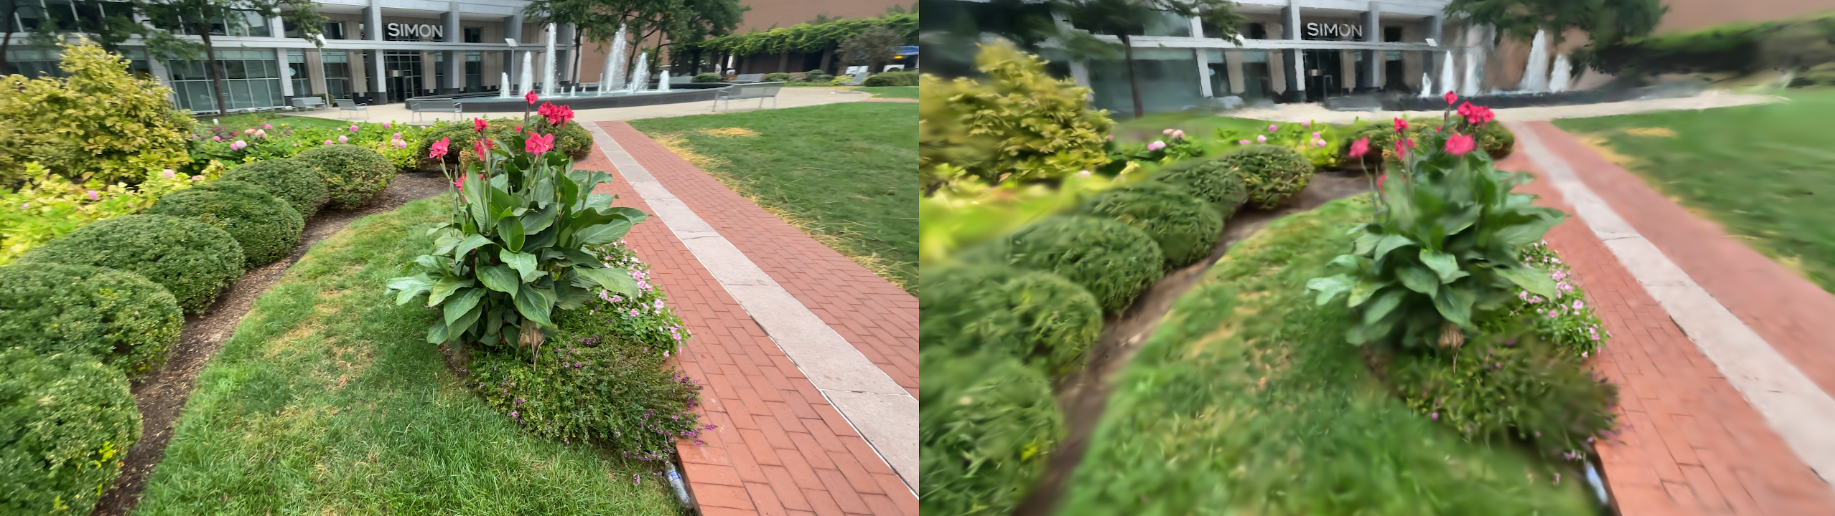
\includegraphics[width=\linewidth]{images/val_step1999_0010.png}
    \caption{Iteration 1}
  \end{minipage}
  \hfill
  \begin{minipage}{0.45\textwidth}
    \centering
    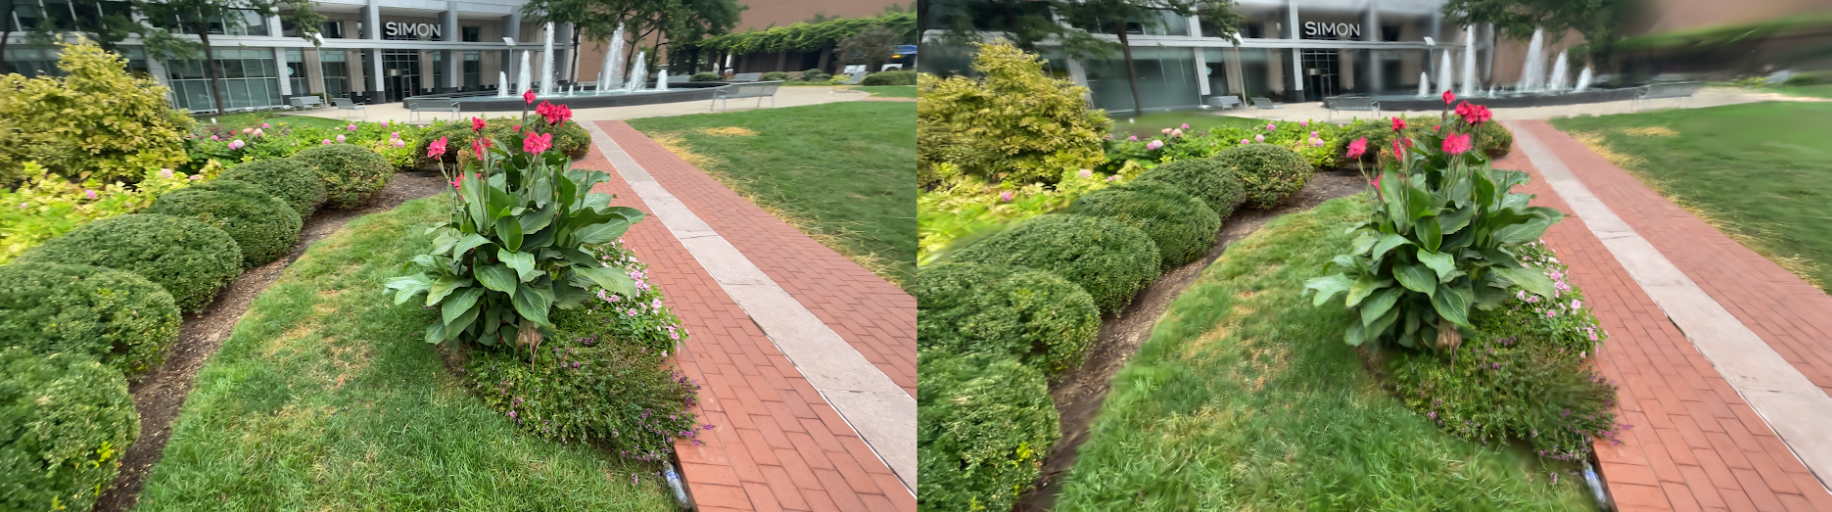
\includegraphics[width=\linewidth]{images/val_step29999_0010.png}
    \caption{Iteration 2}
  \end{minipage}
  \hfill
  \begin{minipage}{0.45\textwidth}
    \centering
    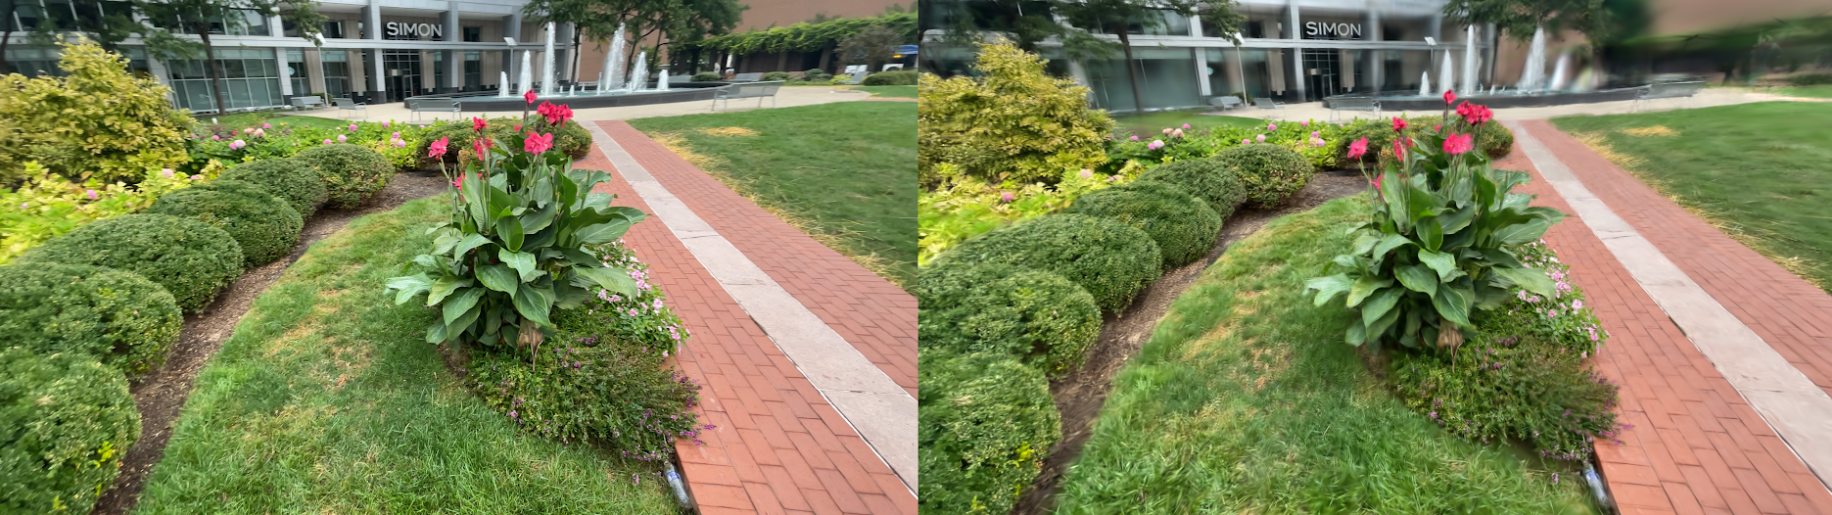
\includegraphics[width=\linewidth]{images/val_step39999_0010.png}
    \caption{Iteration 3}
  \end{minipage}
  \caption{Rasterized Views of the Edited Default Gaussian Splatting per Agentic Loop}
  \label{fig:agentic_views}
\end{figure}

\noindent In Figure \ref{fig:agentic_views}, at iteration 1, we see that the GS reconstruction has severe blur and pervasive clouding. At iteration 2 and 3, we see a significant improvement with the GS having less blurring and clearer reconstruction. Additionally, we can see the improvement per iteration as PSNR and SSIM is increases considerably and LPIPS is reduced significantly, as desired. It is also important to note that the quality of the reconstruction will increase with an increased number of Gaussian points.\\

\noindent In an effort to mitigate the Actor agent from maximizing the training steps and maximum number of Gaussians, we modified the prompt for this experiment to instruct the Actor agent to only increase these two parameters in small increments, and to only do so when necessary. Despite this, the Actor agent still increased the number of training steps from 2,000 to 30,000 between iterations 1 and 2. Although this paper argues for applying agentic workflows to repetitive tasks, our main takeaway from this is that agentic workflows are inherently very time and memory consuming, and should not be left unchecked without human supervision.



